\documentclass[10pt]{article}

\usepackage[a4paper,margin=0.2in]{geometry}
\usepackage{fontspec}
\usepackage{listings}
\usepackage{color}
\usepackage[framemethod=TikZ]{mdframed}
\usepackage[parfill]{parskip}
\usepackage{hyperref}
\usepackage{graphicx}

\setmainfont{Fira Sans}
\setmonofont{Fira Mono}
\newfontface\BoldMonoFont{Fira Mono Bold}[]

\pagenumbering{gobble}

\definecolor{gray}{RGB}{34, 34, 34}
\definecolor{red}{RGB}{248, 103, 78}
\definecolor{carminepink}{rgb}{0.92, 0.3, 0.26}
\definecolor{darkelectricblue}{rgb}{0.33, 0.41, 0.47}
\definecolor{antiquewhite}{rgb}{0.98, 0.92, 0.84}
\definecolor{columbiablue}{rgb}{0.61, 0.87, 1.0}
\definecolor{cadmiumgreen}{rgb}{0.0, 0.42, 0.24}
\definecolor{cobalt}{rgb}{0.0, 0.28, 0.67}
\definecolor{darkorange}{rgb}{1.0, 0.55, 0.0}
\definecolor{grannysmithapple}{rgb}{0.66, 0.89, 0.63}
\definecolor{atomictangerine}{rgb}{1.0, 0.6, 0.4}

\hypersetup{unicode=true,
            colorlinks=true,
            urlcolor=cobalt,
            breaklinks=true}

\lstset{
    inputencoding=utf8,
    extendedchars=true,
    aboveskip=0.5em,
    backgroundcolor=\color{white},
    basicstyle=\normalsize\ttfamily\color{black},
    breakatwhitespace=false,
    breaklines=true,
    captionpos=b,
    escapeinside={\%*}{*)},
    keywordstyle=\BoldMonoFont\color{carminepink},
    identifierstyle=\color{black},
    stringstyle=\color{cadmiumgreen},
    commentstyle=\color{darkelectricblue},
    showspaces=false,
    showstringspaces=false,
    showtabs=false,
    stepnumber=2,
}

\mdfsetup{
    nobreak=true,
    outerlinewidth=0,
    innerlinewidth=0,
    outerlinecolor=red!90,
    innerlinecolor=red!90,
    roundcorner=4pt,
    leftmargin=3,
    rightmargin=3,
    backgroundcolor=white,
    innertopmargin=0,
    innerbottommargin=10,
    innerleftmargin=9,
    innerrightmargin=9,
    splittopskip=\topskip,
}


\pagecolor{atomictangerine!50}

\begin{document}

\twocolumn[
    \begin{@twocolumnfalse}
        \begin{mdframed}
            \begin{minipage}{22.7em}
                \vspace{1.0em}
                {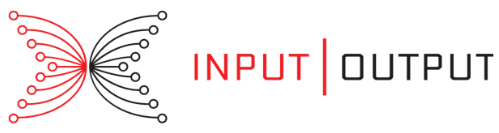
\includegraphics[scale=0.7]{tex/img/iohk-logo.png}}
            \end{minipage}
            \begin{minipage}{27.9em}
                \vspace{0.95em}
                \Large{MONITORING}
            \end{minipage}
            \begin{minipage}{2.5em}
                \vspace{1.0em}
                \href{https://github.com/input-output-hk/iohk-monitoring-framework}{GitHub}
            \end{minipage}
        \end{mdframed}
        \vspace{0.75em}
    \end{@twocolumnfalse}
]

\begin{mdframed}
\section*{\href{https://github.com/input-output-hk/iohk-monitoring-framework/blob/master/iohk-monitoring/src/Cardano/BM/Backend/Monitoring.lhs}{Monitoring}: idea}

    The core idea of monitoring is an ability to monitor some \textit{event} and perform corresponding \textit{action} if that event occurred.
\end{mdframed}

\begin{mdframed}
\section*{Configuration}

Monitoring can be configured in the Yaml configuration file, in the section \texttt{mapMonitors}:

\begin{lstlisting}[language=bash]
  mapMonitors:
    chain.creation.block:
      monitor: ...
      actions:
        - ...
        - ...
\end{lstlisting}

In this example "chain.creation.block" is a logger name, and we will monitor messages sent to this logger.

\end{mdframed}

\begin{mdframed}
\section*{Event}

Monitoring event is defined in the configuration as a logical expression, for example:

\begin{lstlisting}[language=bash]
  monitor: (monitMe >= (42))
\end{lstlisting}

So if the value of \texttt{monitMe} will reach 42 - event occurs.

It's possible to use the following compare operators: \texttt{<=}, \texttt{<}, \texttt{>=}, \texttt{>}, \texttt{==}, \texttt{!=}, \texttt{/=}.

\subsection*{Composition and arithmetic}

Comparisons can be composed using \texttt{And}, \texttt{Or} and \texttt{Not}, for example:

\begin{lstlisting}[language=bash]
  monitor:
    ((monitMe < (2)) Or (monitMe >= (4)))
\end{lstlisting}

It's possible to do basic arithmetic in comparisons using operators \texttt{+}, \texttt{-} and \texttt{*}, for example:

\begin{lstlisting}[language=bash]
  monitor: (monitMe > ((19) * (133)))
\end{lstlisting}
\end{mdframed}

\begin{mdframed}
\section*{Measurable}

Any \href{https://github.com/input-output-hk/iohk-monitoring-framework/blob/master/iohk-monitoring/src/Cardano/BM/Data/Aggregated.lhs}{Measurable} value can be used in comparisons, for example:

\begin{lstlisting}[language=bash]
  monitor: (time > (22 s))
\end{lstlisting}

or

\begin{lstlisting}[language=bash]
  monitor: (f.size > (22 MB))
\end{lstlisting}

Here \texttt{s} corresponds to \texttt{Seconds} and \texttt{MB} to megabytes.
\end{mdframed}

\begin{mdframed}
\section*{Action}

When monitoring event occurred, corresponding action is performing.

Action is defined in the configuration, for example:

\begin{lstlisting}[language=bash]
  actions:
    - CreateMessage Warning "Alert msg!"
\end{lstlisting}

The following actions are supported:

\begin{enumerate}
  \item \texttt{CreateMessage} --- creates a message with defined log severity.
  \item \texttt{SetGlobalMinimalSeverity} --- sets global minimal log severity.
  \item \texttt{AlterSeverity} --- alters log severity for particular logger.
\end{enumerate}
\end{mdframed}

\begin{mdframed}
\section*{Precondition}

It's possible to define precondition expression for monitoring. This precondition is optional, but if it's defined --- monitoring will be performed only if precondition returns \texttt{True}. For example:

\begin{lstlisting}[language=bash]
  monitor-if: (monitMe.fcount >= (10))
  monitor: (monitMe >= (34))
\end{lstlisting}

In this case the first 10 \texttt{monitMe} values will be skipped for monitor analysis.

Please note that technically precondition expression is the same one as an event expression, and can contain the same compare operators, logical compositions and arithmetic operators.

\end{mdframed}

\end{document}
